\chapter{Metodología}
\section{Levantamiento de información}
El departamento de ingeniería mecánica en el Campus Casa Central, posee una máquina de fatiga (MF) uniaxial en flexión en el laboratorio de tecnología mecánica que se encuentra en la universidad hace más de 50 años, sin saber su fecha exacta de adquisición. La medición de fatiga es realizada a través del método de \textit{esfuerzo-vida}, utilizando la configuración de \textit{rotating bending}, ambos descritos en el capítulo anterior. La información existente sobre la máquina de ensayos es escasa, principalmente por su antigüedad, la perdida de documentos y obsolescencia de la electrónica. Por lo mismo, parte del trabajo de esta memoria se centra en lograr rescatar información y su posterior comprensión para lograr tener operativa la máquina de fatiga.

\begin{figure}
\centering
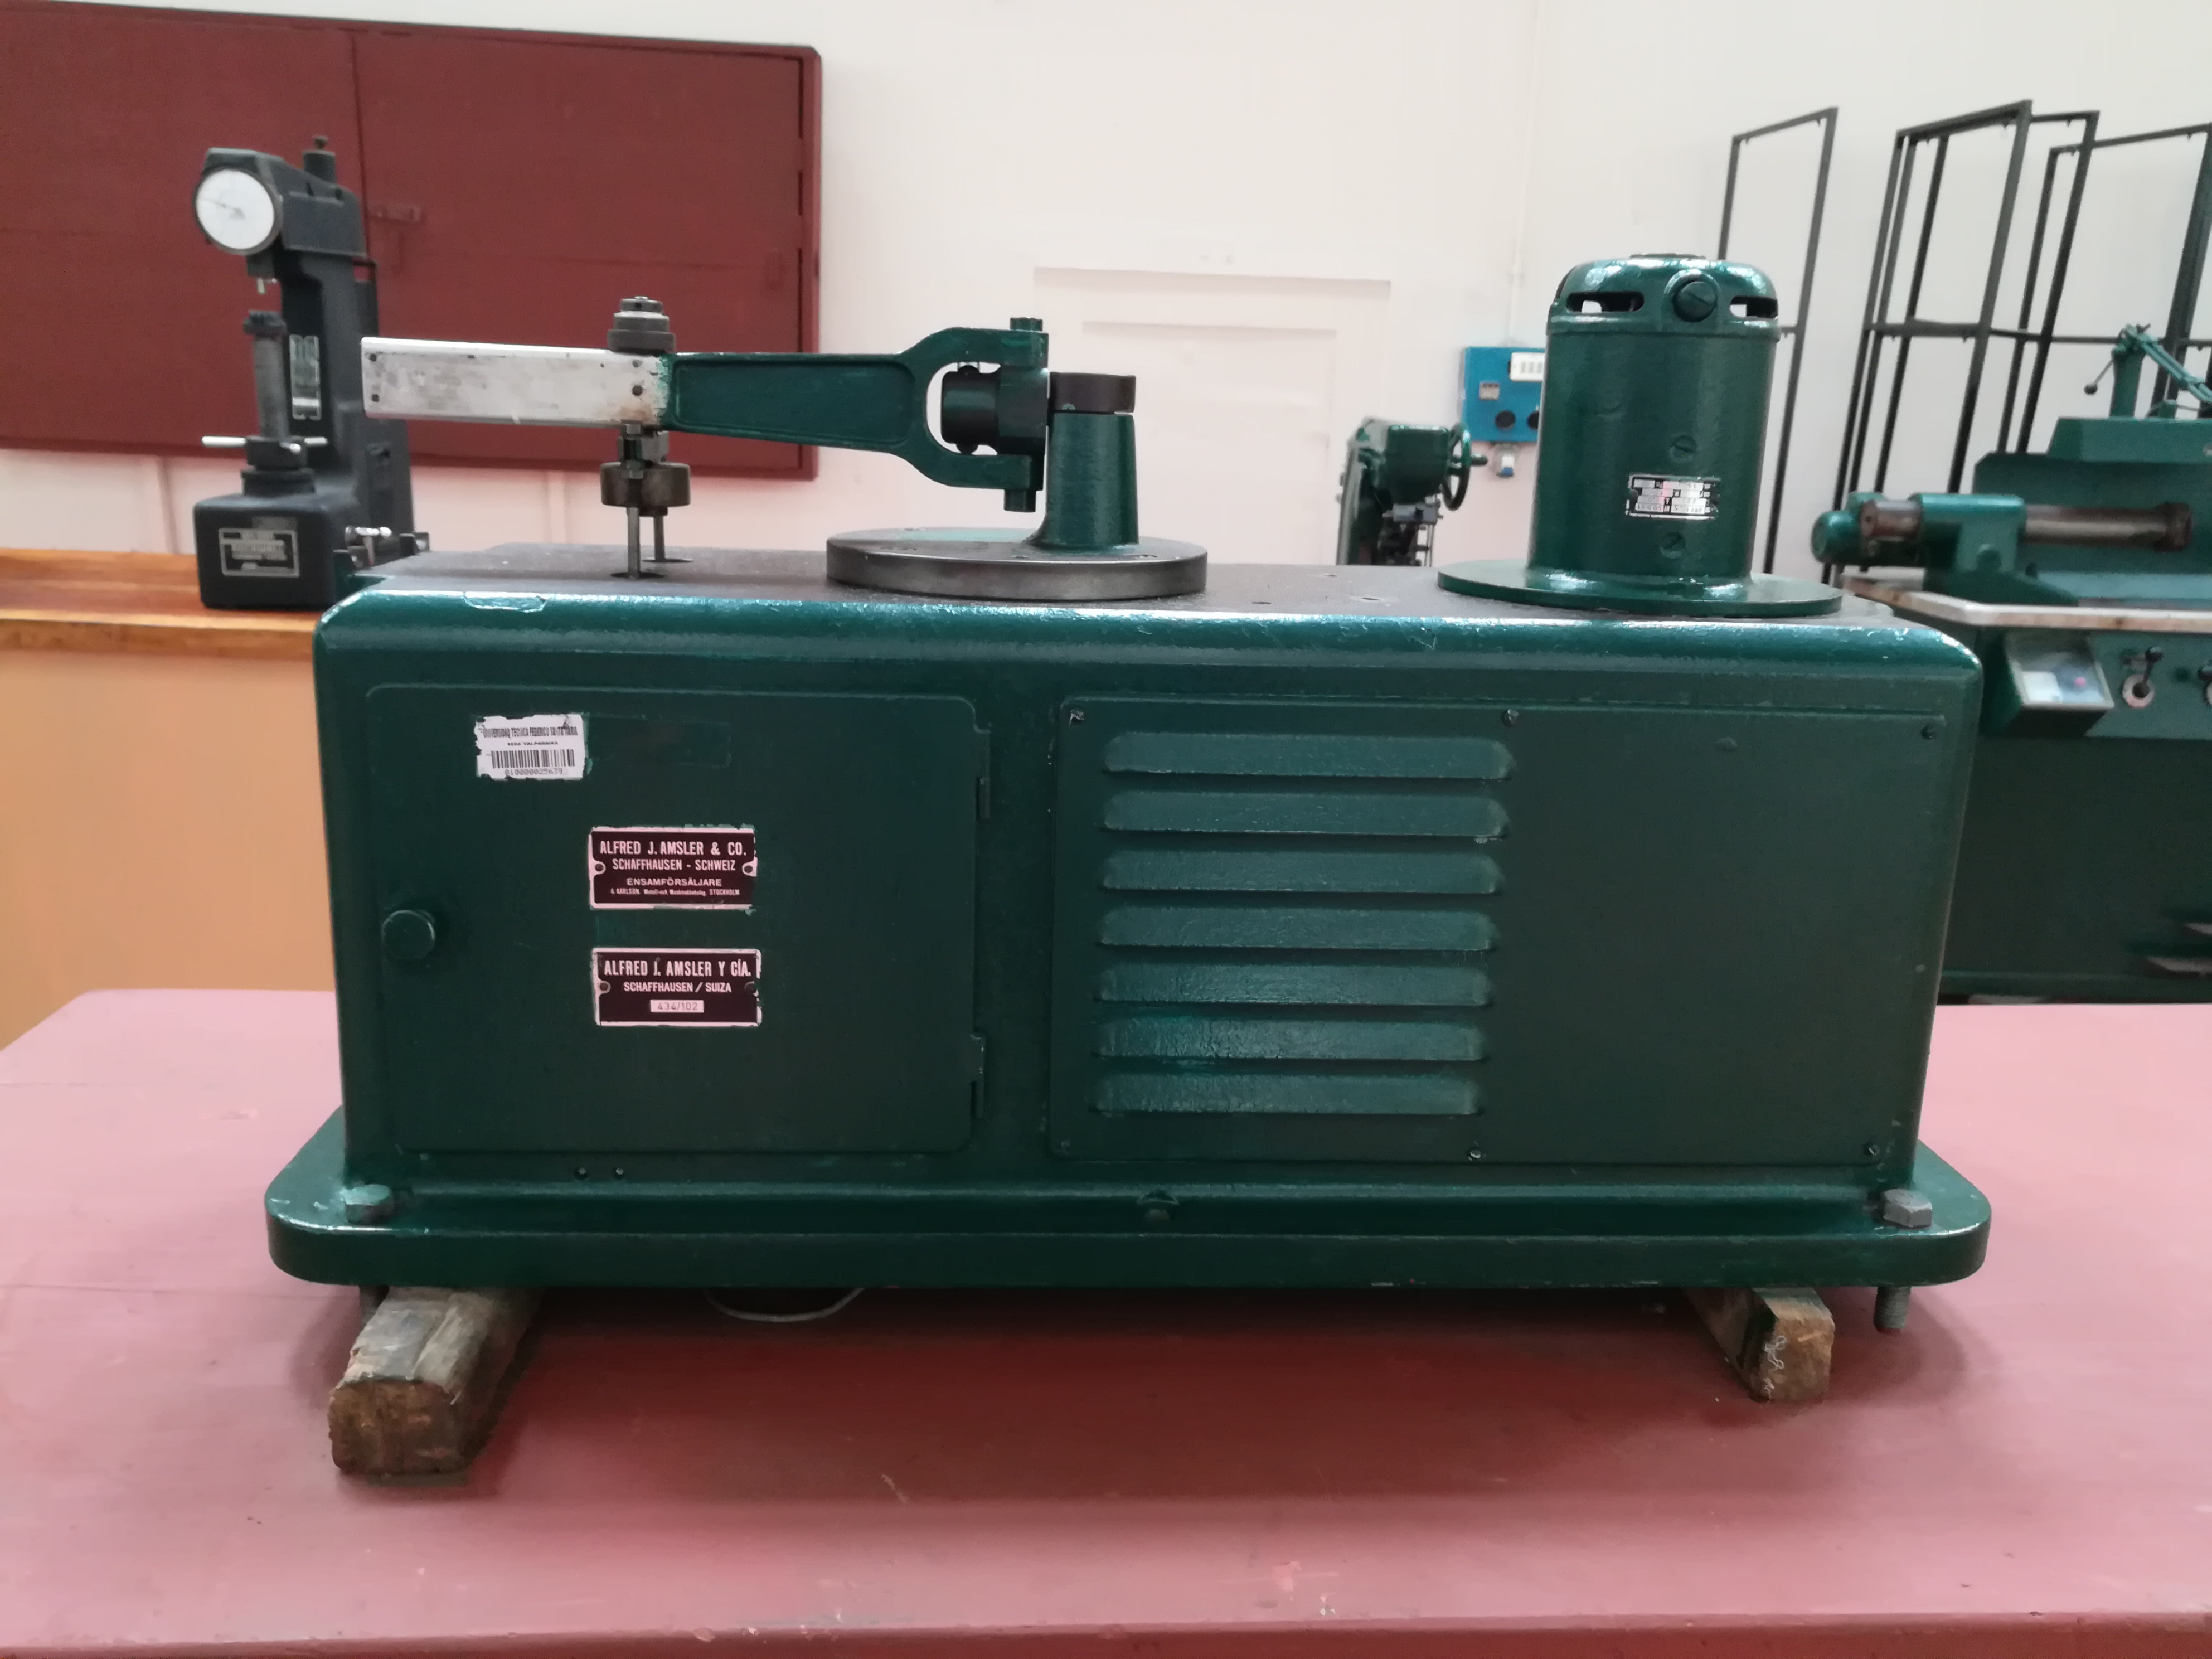
\includegraphics[scale=0.05]{Imagenes/maq_del.jpg}
\label{fig:maq_del}
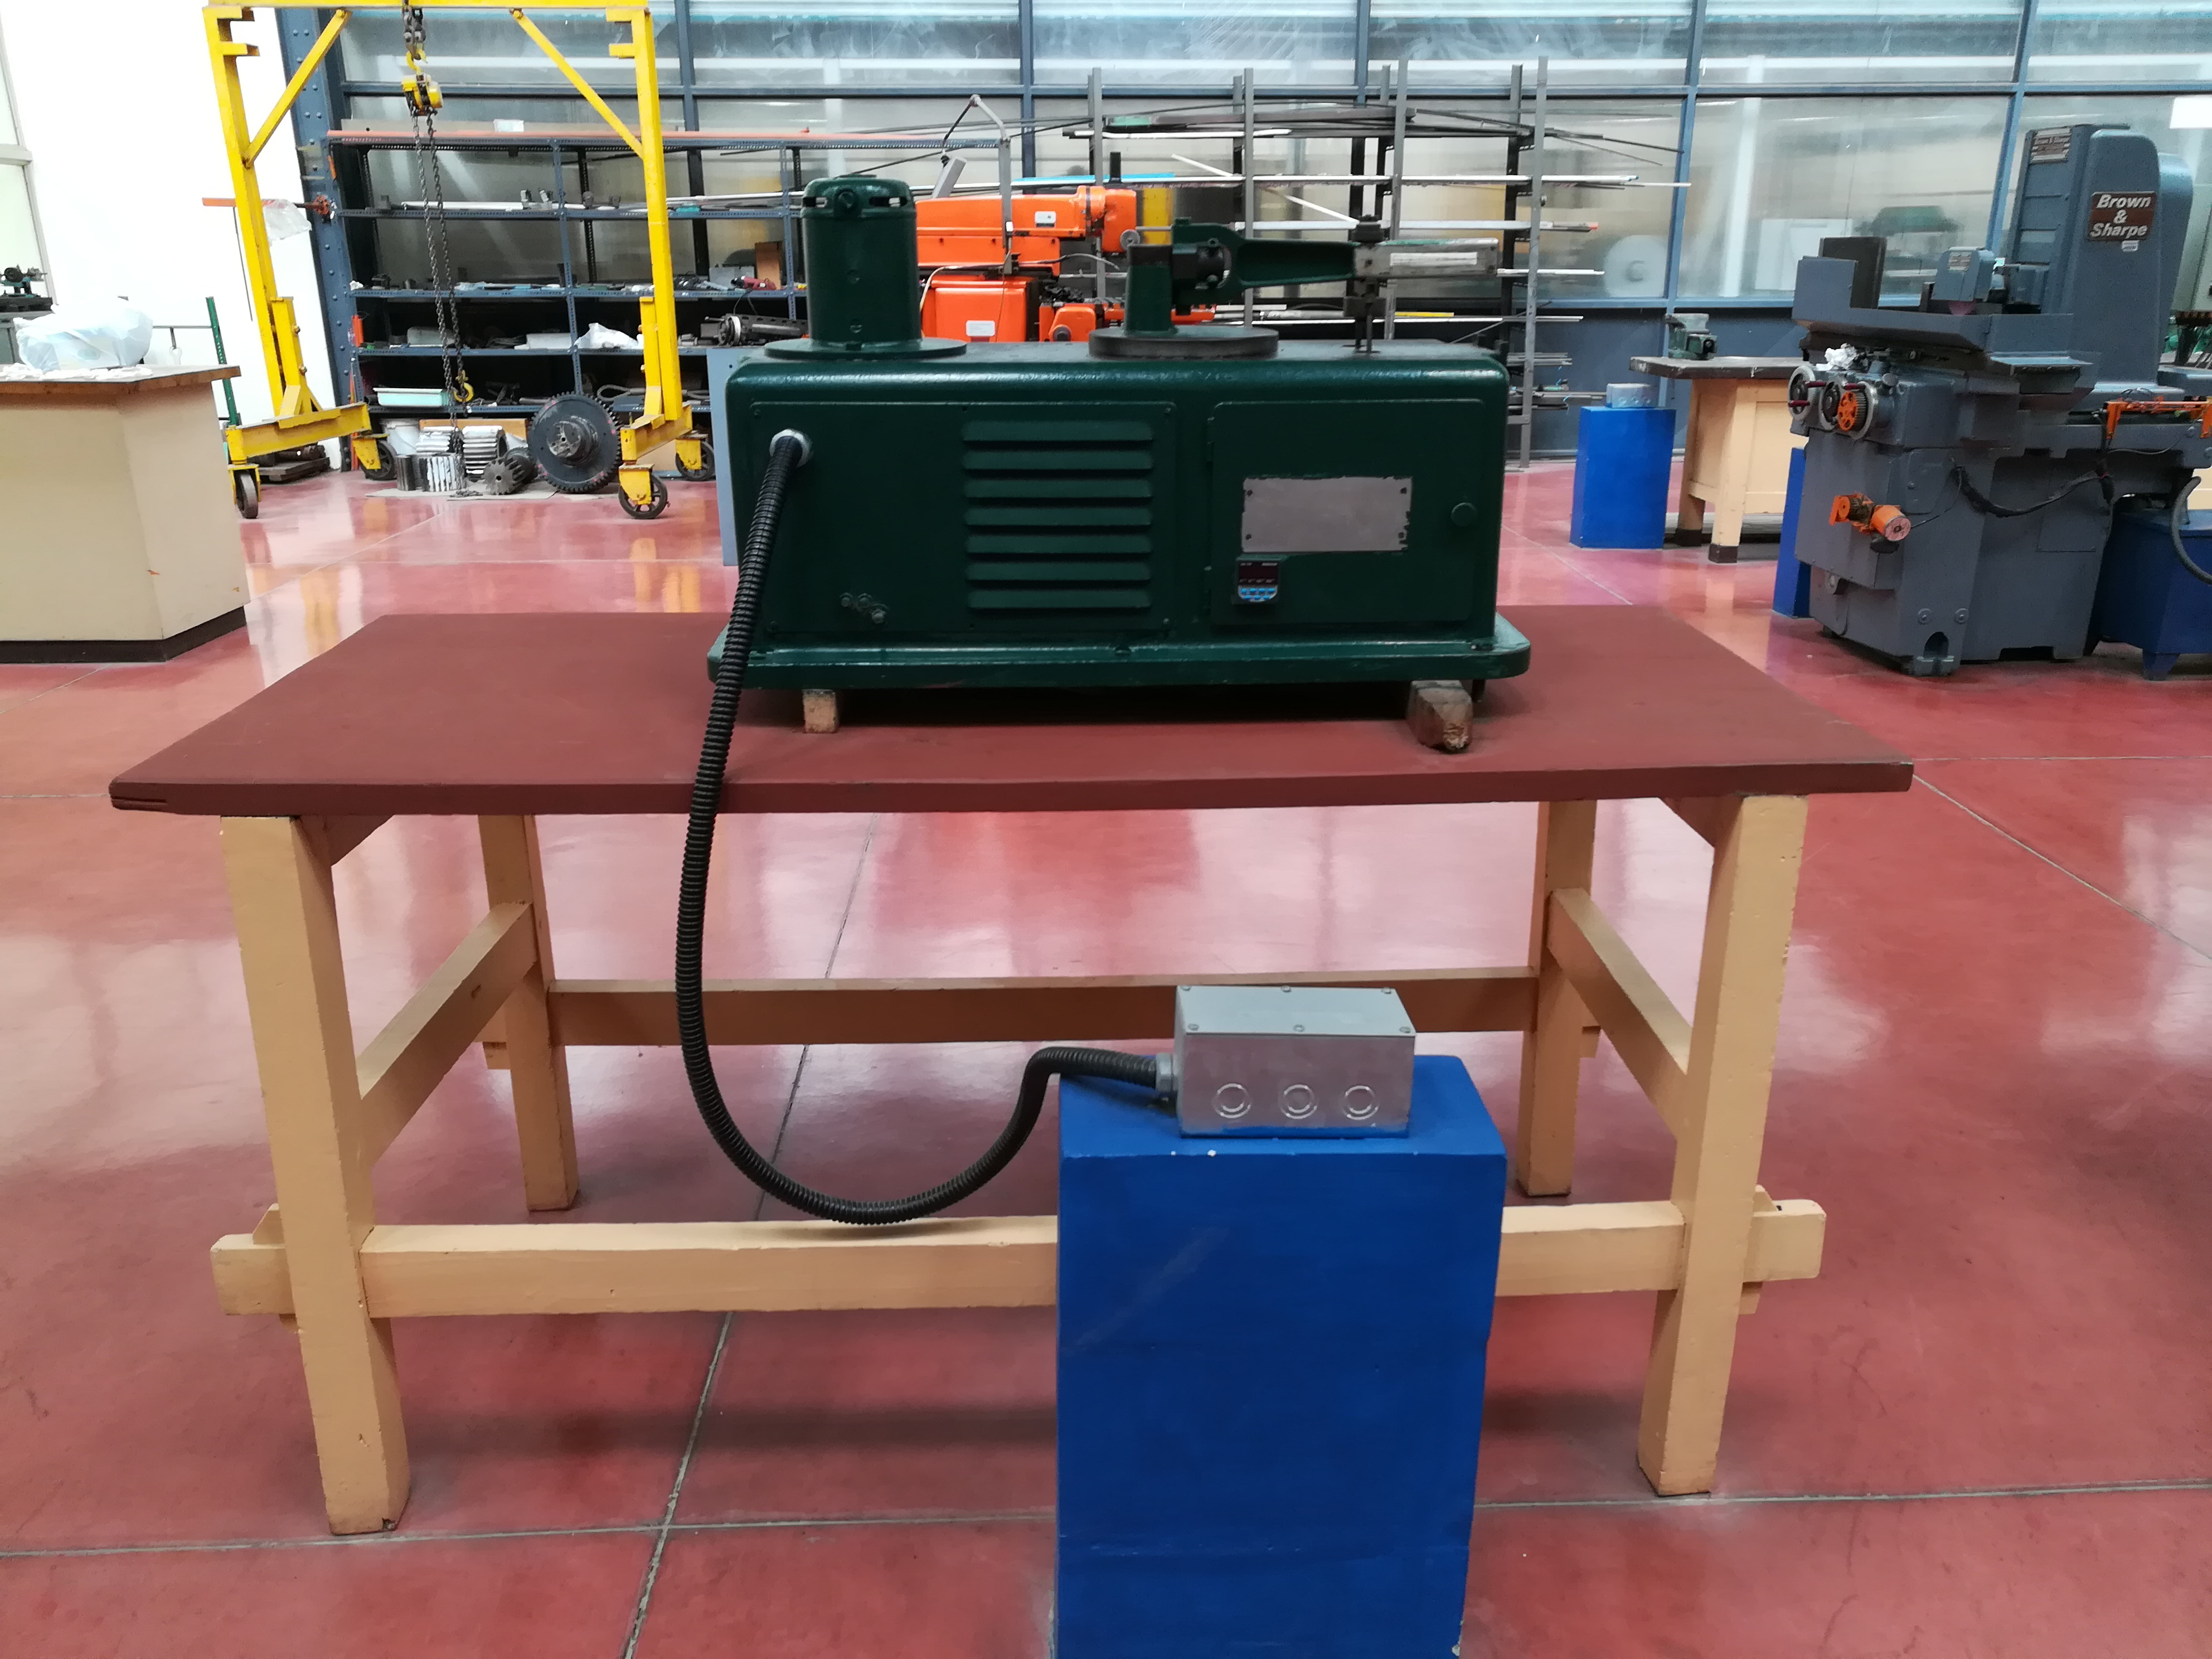
\includegraphics[scale=0.05]{Imagenes/maqfull_post.jpg}
\label{fig:maqfull_post}
\caption{Máquina de fatiga en flexión en el laboratorio de tecnología mecánica}
\label{fig:maq_fat}
\end{figure}


\subsection{Estado actual y antecedentes}
Actualmente la máquina no puede ser utilizada por no estar anclada, estando apoyada sobre dos listones de madera, que a su vez, están sobre una mesa de madera como se aprecia en la figura REF. Por consiguiente, la máquina al ser utilizada comienza a vibrar, saltar y desplazarse lateralmente, lo que impide su uso prolongado por motivos de seguridad. Es decir, no es posible realizar correctamente un ensayo de fatiga de ningún material ni configuración.

A partir de información verbal entregada por el profesor Fernando Rojas, se cree que la máquina fue adquirida por el departamento hace, al menos, 50 años atrás. Fue fabricada en Suiza por \textit{Alfred J. Amsler \& Co.} y su estructura completa es de acero fundido. Previo a la modificación actual del laboratorio, la máquina se encontraba anclada al piso con un bloque de concreto que fue demolido durante la remodelación, momento desde el cual se encuentra sin una solución definitiva. Más aún, varios equipos y máquinas de ensayo del laboratorio no se encuentran ancladas al piso ni con una instalación definitiva impidiendo su uso.

La única modificación que posee la máquina, según la información recopilada, consiste en el cambio del contador de revoluciones o ciclos realizados en un ensayo de fatiga. Esta actualización consistió en sacar el contador mecánico original y reemplazarlo por un contador electrónico, el cual tiene sus controles y el display adosada a su estructura, como se puede apreciar en la figura \textcolor{red}{agregar imagen del contador}. 

El sistema eléctrico de la máquina permanece intacto, la cual se encuentra conectada a la red de la universidad. Conserva su motor eléctrico original junto a un conjunto eléctrico cuya función es suministrar energía de manera continua y estable al motor, para evitar que el ensayo de fatiga se pueda ver afectado por problemas y las variaciones del suministro eléctrico. El motor es de \textcolor{red}{corriente continua} con velocidad constante y sus especificaciones se pueden ver en la tabla \ref{tab:motor_maq} :
\begin{table}[h]
\centering
\begin{tabular}{ll}
\hline
Especificaciones Motor                            & Valor   				\\ \hline
Tensión                                           & 220 {[}V{]}        		\\
Corriente                                         & 0,8 {[}A{]}        		\\
Factor de potencia ($\cos \varphi$)				  & Sin información    		\\
Potencia                                          & 100 {[}W{]}        		\\
Velocidad                                         & 1500 {[}rev/min{]} 		\\ \hline
\end{tabular}
\caption{Especificaciones del motor de la máquina de fatiga.}
\label{tab:motor_maq}
\end{table}

Otro elemento distinto al original consiste en la correa de transmisión entre el motor eléctrico y el disco desbalanceado. La original consistía en una correa de cuero plana y cruzada, sin información respecto a su empalme. La correa actual consiste también en una correa plana y cruzada, sin embargo, su material es tela y el empalme es realizado a mano con hilo acerado. Cabe destacar que lo poco usual de las dimensiones, características y la necesidad de hacer el empalme en la misma máquina, dificulta la búsqueda de una correa que pueda cumplir de manera óptima la transmisión de potencia. Parte de estas dificultades se deben a que el sistema de transmisión no ha sido modificado donde sus poleas tienen dimensiones, tanto de diámetro como de ancho, que no están normalizadas o se encuentran fuera de catálogo de mucho proveedores. 

Por otro lado, los elementos de agarre de la probeta no tienen modificaciones conocidas, tanto el brazo que recibe el movimiento como el agarre empotrado a la estructura de la máquina. La fabricación de las probetas utilizadas se realiza en el mismo laboratorio a partir de acero AISI 1020 o 1040, el cual para conseguir las dimensiones de la figura REF. se debe cortar y tornear.

Finalmente, para realizar los ensayos en distintas configuraciones existen distintas masas (figura REF) que desequilibran el disco rotativo, como se verá en la sección \ref{sec:funcionamiento}, y estas combinaciones se especifican en una tabla de cargas (Anexo REF). Sin embargo, se desconoce el origen, y en consecuencia, la fiabilidad de la información contenida en esta tabla.

\subsection{Funcionamiento}
\label{sec:funcionamiento}
La máquina de fatiga tiene como objetivo lograr que para cada ciclo se ejerza el mismo esfuerzo determinado sobre la probeta, en forma de flexión. Para lograr esto, el mecanismo utilizado es un disco desequilibrado girando a una velocidad constante $\dot{\theta}$, la fuerza es transmitida hasta un brazo que sostiene a su vez a la probeta, generando flexión en la probeta con un doble empotramiento. La velocidad $\dot{\theta}$ del disco se transmitida desde el motor eléctrico a través de poleas y una correa de transmisión en una relación de 1:1 \textcolor{red}{revisar}, a una velocidad de 1500 revoluciones por minuto. Así, para realizar las mediciones de fatiga a distintas cargas se modifica el desequilibrio del disco a través de un conjunto de masas, mostradas en la figura \ref{fig:contrapesos}, que permiten generar distintas configuraciones y, por consiguiente, esfuerzos en la probeta. 

\begin{figure}
\centering
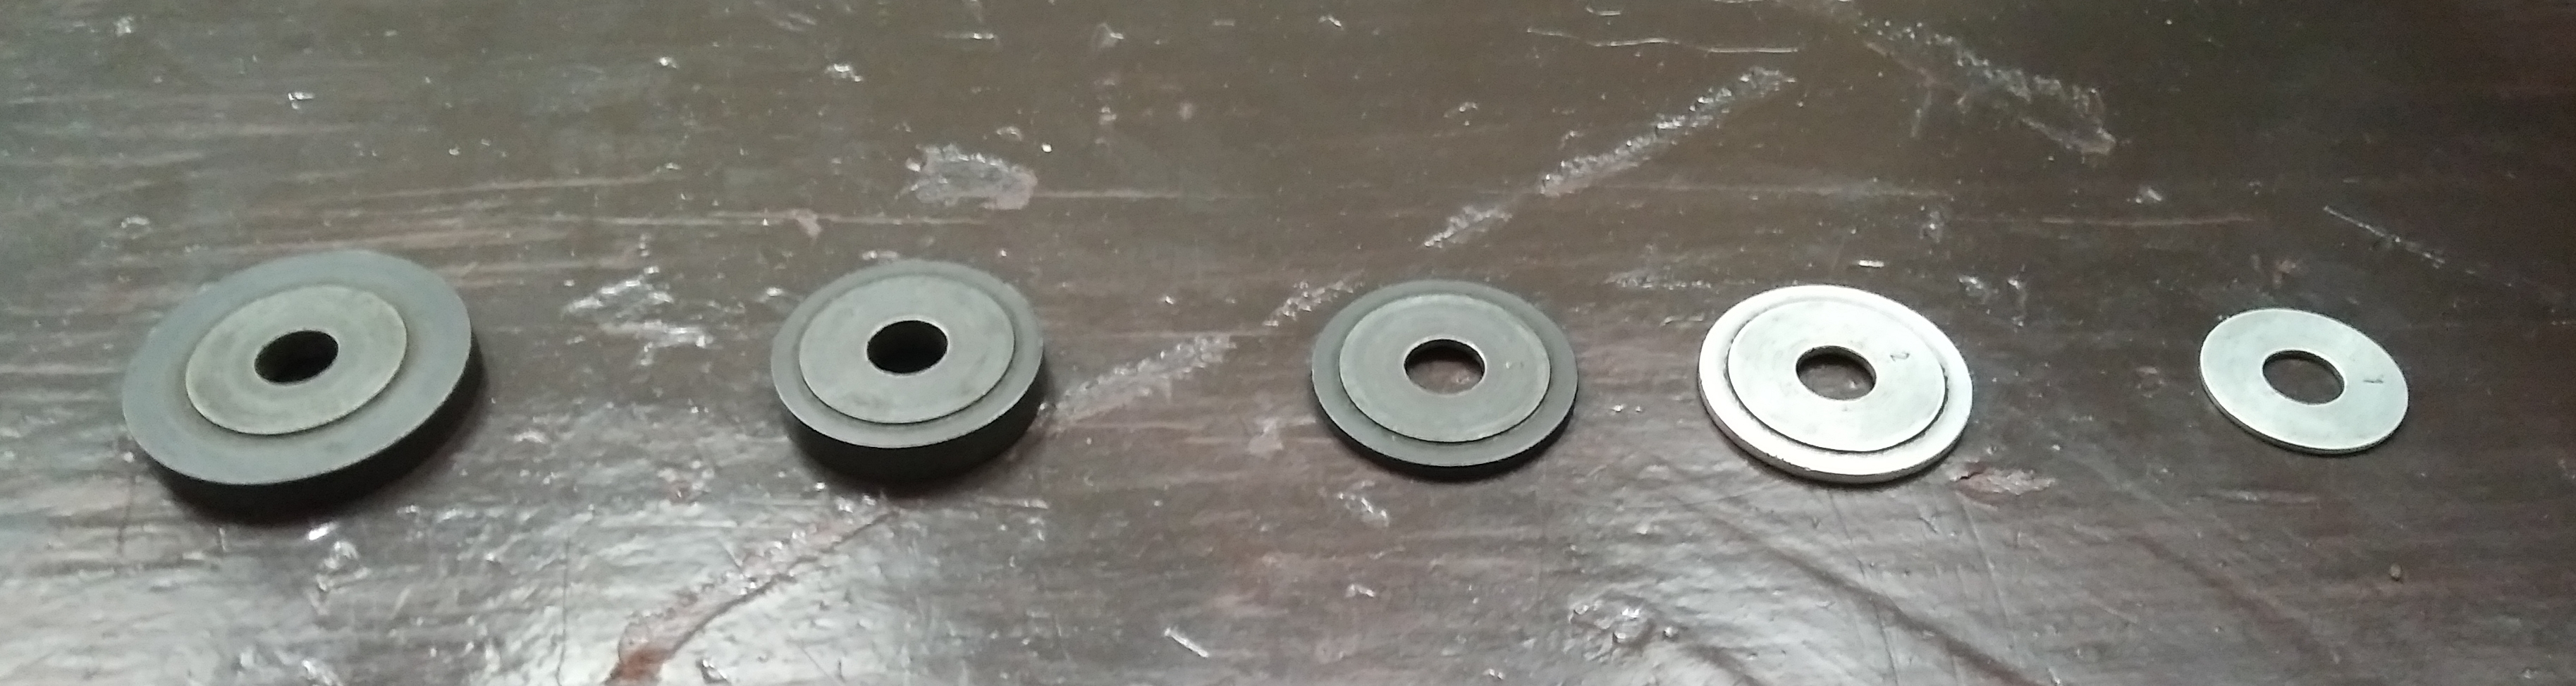
\includegraphics[scale=0.11]{Imagenes/contrapesos.jpg}
\caption{Contrapesos utilizados para desequilibrar el disco, ordenados desde el 5 hasta el 1 de izquierda a derecha.}
\label{fig:contrapesos}
\end{figure}


Los elementos utilizados para desbalancear son 6 discos pequeños de X \textcolor{red}{medir radio masas} a Y de diámetro. Estos son enumerados del 1 al 5, donde el 1 es el más liviano y el 5 el más pesado, todos de distinto peso y el quinto se encuentra repetido. Estas se colocan en los extremos del disco giratorio, como se ve en la figura REFimagendisco, dependiendo de la carga que se desee generar. Para conocer que configuración corresponde a cada esfuerzo aplicado sobre la probeta, se utiliza la tabla de cargas explicada a continuación.

Esta tabla, con 3 columnas de información como se ve en el Anexo REF, nos entrega el esfuerzo normal $\sigma$, cortante $\tau$ y la combinación necesaria para generar esos esfuerzos. Los números entre paréntesis nos indican cuantos contrapesos se deben apilar en cada perno adosado al disco giratorio, los cuales llamaremos soportes de contrapeso (SC). Así, la tabla nos señala que la fuerza es función de la diferencia de masa entre cada soporte, es decir, la suma de las masas de cada paréntesis. A modo de ejemplo, en la tabla \ref{tab:ejemplo_config} se han colocado las 4 primeras filas de la tabla de cargas, añadiendo 4 columnas con información sobre el peso de cada combinación. En las columnas $m_1$ y $m_2$ se aprecia la suma de cada masa colocada en sus soportes de contrapeso señalado por la columna de ``Combinación''. Las columnas siguientes representan $\Delta m = m_1-m_2$ y $m_{total}=m_1+_2$. Como se puede apreciar, los esfuerzos normales y cortantes aumentan en la medida que $\Delta m$ de cada combinación aumenta, independiente de $m_{total}$.

\begin{table}[h]
\centering
\label{tab:ejemplo_config}
\begin{tabular}{@{}cclllll@{}}
\toprule
$\sigma \left[\frac{\text{kg}_f}{\text{cm}^2}\right]$ & {$\tau \left[\frac{\text{kg}_f}{\text{cm}^2}\right]$} & Combinación     & $m_1$ {[}g{]} & $m_2$ {[}g{]} & $\Delta m$ {[}g{]} & $m_{total}$ {[}g{]} \\ \midrule
40                                                   & 20                                                                    & (5) - (1+2+3+4) & 30,9199       & 30,5071       & 0,4128             & 61,427              \\
80                                                   & 40                                                                    & (1) - (0)       & 0,7582        & 0             & 0,7582             & 0,7582              \\
120                                                  & 60                                                                    & (5) - (4+2+3)   & 30,9199       & 29,7489       & 1,171              & 60,6688             \\
160                                                  & 80                                                                    & (2) - (1)       & 2,2969        & 0,7582        & 1,5387             & 3,0551              \\ \bottomrule
\end{tabular}
\caption{Tabla de configuración de las masas modificada, mostrando el peso, su diferencia y el total para cada combinación}
\end{table}

Con esto, la probeta a ensayar estará sometida a un esfuerzo en flexión, empotrada en ambos lados por la mordaza del brazo y la mordaza empotrada a la estructura de la máquina, ambas mostradas en la figura \ref{fig:grippers}. Una vez que se haya escogido la configuración de masas y la probeta se encuentre en su posición, una pequeña barra con una manilla ubicada entre las barras de acero, como se aprecia en la figura REF, eleva ambas barras con el objetivo de evitar que oscile durante el encendido y aceleración del motor hasta su velocidad final, dejando a la barra en una configuración de empotrado y apoyo simple. Una vez que el motor alcanza una velocidad estable, el sostén es girado nuevamente para dejar al disco giratorio en posición de empotrado-libre. Este sostén, permite que el ensayo de fatigue se realice siempre a una frecuencia constante y evitar la transición inicial del motor. Una vez que la probeta se fracture, provocarán un aumento en la amplitud de las oscilaciones del disco las cuales activarán el freno automático (figura REF) para detener el motor y, por lo tanto, el ensayo. Gracias a este sistema, es posible conocer la cantidad de ciclos que realizados hasta el momento de fractura sin la necesidad de supervisar de manera continua el ensayo.

\begin{figure}
\centering
\includegraphics[scale=0.08]{Imagenes/mordazas.jpg}
\caption{A la izquierda se puede apreciar la mordaza adosada al brazo y a la derecha la mordaza fija.}
\label{fig:grippers}
\end{figure}

\subsection{Mediciones}
Para realizar un correcto diseño de la estructura soportante y la compresión de su funcionamiento, se hace vital poder contar con información confiable para obtener resultados correctos. Para esto, las mediciones se dividirán según su objetivo en el desarrollo de este trabajo.
\subsubsection{Diseño de estructura}
Las medidas de la mesa actual son: 
\begin{itemize}
	\item Ancho = 74,5 cm
	\item Largo = 177 cn
	\item Altura = 91 cm
\end{itemize}
Por otro lado, para diseñar correctamente la estructura se deben conocer las dimensiones de la máquina, su peso y la ubicación de los pernos de anclaje, así como también el tipo de perno utilizado. La figura REF\textcolor{red}{realizar diagrama con vistas frontal y lateral de la maquina con sus dimensiones} es un esquema representativo de la máquina, mostrando sus dimensiones de ancho, alto y largo, las dimensiones de su base y la ubicación de sus pernos. La masa de toda la máquina se aproximó a partir de las dimensiones externas, estimando el grosor de sus paredes y considerando el peso específico del acero fundido, sobrestimando el valor del espesor de sus paredes como factor de seguridad. Considerando el peso específico del acero $\rho_{acfund} = 7850 \, [Kg/m^3]$, entonces la masa total calculada es:
\[ \left.
\begin{array}{ll}
V_{base} &= (3,3\cdot91\cdot39 - 3,3\cdot88\cdot37)\;\text{cm}^3		\\
V_{superior} &=(30,2\cdot84\cdot32 - 26\cdot78\cdot28,5)\; \text{cm}^3 \\
\end{array}
\right\} \\
\quad V_{b+s} = 24345,9 \; \text{cm}^3 \]
\begin{equation}\label{eq:masa_maquina}
	m_{maq} = \rho \cdot V_{b+s} = 191,1 \: kg \approx 200 \: kg
\end{equation}
El peso total de la máquina es aproximado a 200 kg como un factor de seguridad al momento de diseñar los elementos de la nueva estructura.

\subsubsection{Caracterización de los componentes}
\subparagraph{Sistema de transmisión}
El sistema de transmisión está compuesto por el motor eléctrico, cuyas características se detallaron anteriormente, la correa de transmisión y ambas poleas. Las dimensiones y características de las poleas conductora y conducida, como también de la correa se encuentran en la tabla \ref{tab:transmision}. %Además, la figura REF y REF, muestran el estado actual de la correa de transmisión y la ubicación del motor eléctrico.
\begin{table}[]
\begin{tabular}{@{}ll@{}}
\centering
\toprule
Caracteristicas           & Valor   \\ \midrule
Diametro polea conductora & 60 mm   \\
Diametro polea conducida  & 49 mm   \\
Ancho correa              & 10 mm   \\
Longitud correa           & 1235 mm \\
Configuración             & Cruzada \\ \bottomrule
\end{tabular}
\caption{Datos del sistema de transmisión}
\label{tab:transmision}
\end{table}

\subparagraph{Barras de acero}
El conjunto de barras de acero que sostienen el disco en empotrado-libre, tienen medidas levemente distintas para las superiores respecto a las inferiores, separadas por una distancia de 32 mm. La tabla \ref{tab:medidas_barrasacero} muestra las medidas de cada una.
\begin{table}[h]
\centering
\label{tab:medidas_barrasacero}
\begin{tabular}{@{}lll@{}}
\toprule
Medida  & Barras superiores {[}mm{]} & Barras inferiores {[}mm{]} \\ \midrule
Espesor      & 5,7                        & 5,8                        \\
Ancho        & 25,1                       & 25,2                       \\
Largo        & 333                        & 333                        \\ \bottomrule
\end{tabular}
\caption{Medidas de las barras de acero según su posición}
\end{table}

\subparagraph{Sistema de transmisión de fuerzas}
El brazo principal (figura REF) que ejerce la fuerza sobre la probeta proveniente del disco desbalanceado, está constituido por tres partes principales. La primera de ellas es la parte trasera, con forma regular de paralelepípedo, está hecho de una aleación de aluminio y dos tercios de su longitud es ahuecada. La segunda y principal, está hecha de acero fundido y añade el mayor porcentaje de masa al total del brazo. Finalmente, la última parte consiste en la mordaza, unida a la sección principal con dos pernos que permiten ajustar su posición. La longitud total del brazo es de 359 mm y su masa total 2,305 kg

%\begin{figure}
%\centering
%\includegraphics[scale=0.08]{Imagenes/brazo_mordaza.jpg}
%\caption{Brazo de momento de carga}
%\label{fig:brazo_mordaza}
%\end{figure}

La transmisión entre el disco desbalanceado y el brazo se da a través de dos barras de acero, uno a cada lado del disco, de diámetro 6,2 mm y largo de 169 mm. 

\subparagraph{Disco desbalanceado}
En base a las características visuales y auditivas del disco, se cree que está construido en alguna aleación de aluminio. Su radio $R_d =$ 112 mm y espesor de . 

La masa de cada contrapeso, medidos en el laboratorio de metalúrgica con pesas blablabla.
\begin{table}[H]
\centering
\begin{tabular}{@{}cc@{}}
\toprule
Contrapeso & Masa {[}g{]} \\ \midrule
1          & 0,7582       \\
2          & 2,2969       \\
3          & 6,8541       \\
4          & 20,5979      \\
5          & 30,9199      \\ \bottomrule
\end{tabular}
\caption{Masa de cada contrapeso utilizado}
\label{tab:masa_contrapesos}
\end{table}

\section{Diseño de estructura}
El proceso de diseñar la estructura hasta su resultado final pasó por distintas etapas. Esto por el proceso de aprendizaje y comprensión de la norma de calculo de madera NCh 1198, como también por la restricción y disponibilidad de materiales, tecnología o medidas acorde a las necesidades. El diseño presentado en este trabajo se muestra en la figura REF, hecho principalmente de madera, junto a elementos de acero. El objetivo de esta estructura es fijar y soportar la máquina de fatiga tanto en reposo como en operación, buscando como características su durabilidad, lo modular de las piezas y la opción de modificarla en el futuro.

La metodología de su diseño, se separará en las distintas etapas que se realizó y los requerimientos que surgieron a partir de estas. Finalmente, se realizó una simulación estática y modal para comparar los cálculos realizados y conocer su frecuencia natural, respectivamente.

\subsection{Diseño en acero}
La estructura se diseño para que la conexión con la máquina de fatiga fuera a través de placas de acero, utilizando los pernos existentes. Las placas, a su vez , están conectadas mediante pernos a las vigas transversales de madera de cada extremo. Para llevar acabo los cálculo, se hará como suposición que cada placa esta con un empotramiento en cada extremo, con dos cargas distribuidas. La primera de ellas es el apoyo de la maquina sobre la placa y, la segunda, el peso propio del acero. Por lo tanto, la figura REF muestra el diagrama de las cargas que actúan y las distancias a utilizar. 

\textcolor{red}{Diagrama de cargas}

Por otro lado, al no conocerse la distribución de masa de la maquina de fatiga, se considerará la carga distribuida en cada placa como:
\begin{equation}
	 q_{maq} = \frac{0,75\cdot m_{maq}}{c} = 384,62 \; [\text{kg/m}]
\end{equation}
Donde $m_{maq}$ es la masa estimada en \ref{eq:masa_maquina}, multiplicada por 0,75 como factor de seguridad por la distribución irregular de peso de la máquina. Para obtener el esfuerzo máximo flector es necesario conocer la geometría de la viga, motivo por la cual se iteró entre las distintas opciones disponibles en el mercado de placas o barras planas de acero. Por razones estipuladas en la norma NCh 1198, la conexión entre la placa de acero y la viga transversal de madera se debe realizar con un mínimo de dos pernos, por lo tanto, se le dio prioridad al ancho de la placa. Así, la tabla \ref{tab:dimycar_placa} muestra las dimensiones de la placa escogida.
\begin{table}[h]
\centering
\begin{tabular}{@{}ll@{}}
\toprule
Características              & Valor        \\ \midrule
Espesor {[}mm{]}             & 8            \\
Ancho {[}mm{]}               & 100          \\
Material                     & Acero A270ES \\
Carga distribuida {[}kg/m{]} & 6,28         \\ \bottomrule
\end{tabular}
\caption{Dimensiones y características de la viga de acero}
\label{tab:dimycar_placa}
\end{table}

Por ende, el cálculo de la reacción en sus apoyos, el momento y esfuerzo flector máximo queda expresado por las ecuaciones \ref{eq:reaccion_acero}, \ref{eq:mtofleca_acero} y \ref{eq:esfmax_acero}, respectivamente. Estas fueron calculadas respecto al punto $A$ (o $B$, por simetría), donde se encuentra el momento flector máximo.

\begin{subequations}
	\begin{gather}
		R_A = g\left(\frac{m_{maq}}{2} + \frac{q_{ac}L}{2}\right) \label{eq:reaccion_acero}\\ 
		M_A = \left(\frac{-gaq_{maq}}{24L}\right) \left(4b^2 - \frac{6cb^2}{L} + \frac{3b^3}{L} - 3L^2\right) + \left(\frac{gq_{ac}L^2}{12}\right) \label{eq:mtofleca_acero} \\
		\sigma_{max} = \frac{M_A \cdot c}{I} \label{eq:esfmax_acero}
	\end{gather}
\end{subequations}

Así, los valores obtenidos son:
\begin{itemize}
	\item $R_A = 754,85$ [N]
	\item $M_A = 100,97$ [Nm]
	\item $\sigma_{max} = 94,66$ [MPa]
\end{itemize}

\subsection{Diseño en madera}

\subsection{Cálculo de cargas en estructura de madera}

\subsection{Uniones}
\subsubsection{Acero - madera}
\subsubsection{Madera - Madera}
\subparagraph{Pernos}
\subparagraph{Tirafondos}
\subsubsection{Herrajes y conectores}

\subsection{Simulaciones}
\subsubsection{Estática}
\subsubsection{Modal}


\section{Modelo del sistema de funcionamiento}
\subsection{Diagrama del sistema}

\subsection{Modelo del sistema}
\subsubsection{Simplificaciones}
\subsubsection{Modelo del disco desbalanceado}
\subsubsection{Cálculo y obtención de valores del sistema}

\subsection{Ecuaciones de movimiento de la máquina de fatiga}

\subsection{Carga sobre la probeta}

\section{Análisis de información existente}
\subsection{Simulación de cargas}